\subsection{Firing circuit}
The turret needs to run two motors in the gun to properly fire. The mbed can put out small amounts of voltage and very low amounts of current. The motor requires much higher current and voltage than the mbed can supply. So, a firing circuit is used to control the  motors from the mbed, and provide the motors with the proper voltage and current.
\begin{figure}[h!]
    \centering
    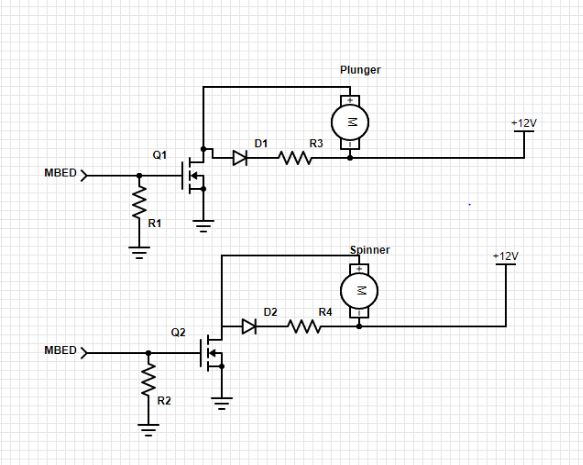
\includegraphics[scale=.5]{fcscheme.JPG}
    \caption{Firing Schematic}
    \label{fig:firing schematic}
\end{figure}

  
\begin{figure}[h!]
    \centering
    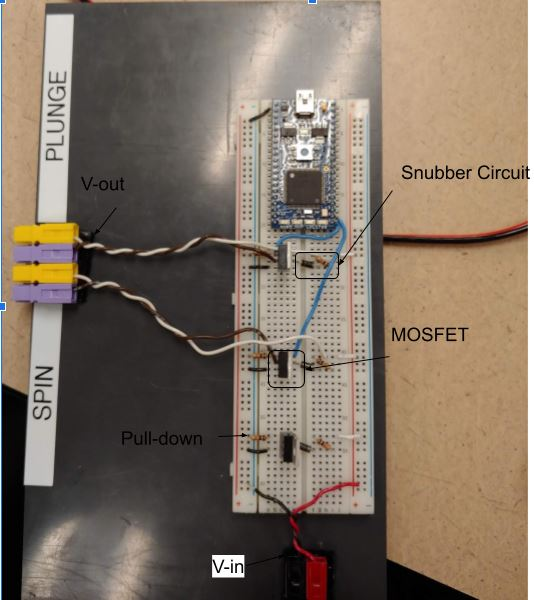
\includegraphics[scale=.4]{firecircuit.JPG}
    \caption{Firing Circuit}
    \label{fig:firing circuit}
\end{figure}

% This part describes how the firing circuit functions
The pulldown resistor is to put a high resistance between the mbed pin and ground. This means that the transistor gate pin is not connected directly to ground, so the transistor will close when the mbed pin is high.
The mbed is incapable of directly driving the motors, but is capable of controlling a mosfet on/off. So, the mosfet functions as a switch, controlled by the mbed, for the motor circuits, allowing the mbed to control otherwise oversized loads.
A motor is a high inductance load. When the mosfet is off, the current produced by the inductive components of the motor needs some way to dissipate. The flyback diode and snubber allow for this induced current to disperse. 

%Statement of Contribution - Ok to leave as comment
%MIDN Malatesta created the first and third (backup) mosfet circuits. Midn Hendricks created the second by copying the first circuit. The overall contribution was roughly 60% Malatesta, 40% Hendricks.